%This is a Latex file.
\documentclass[12pt]{article}
\usepackage{
	latexsym,
	fancyhdr,
	amsmath,
	amsfonts,
	dsfont,
	amsthm,
	amssymb,
	mathrsfs,
	mathtools
}
\usepackage[margin=0.94in]{geometry}
\usepackage{lastpage} % Required to determine the last page for the footer
\usepackage{tikz}
\usetikzlibrary{arrows.meta}
\usepackage{url, hyperref}

\parindent 0pt

\pagestyle{fancy} \lhead{\sf MTH 411} \chead{\sf Homework \#05}
\rhead{\sf Due: Friday 10/23/2018} \lfoot{} \cfoot{} \rfoot{}

\newcommand{\N}{\mathds{N}}
\newcommand{\Z}{\mathds{Z}}
\renewcommand{\vec}[1]{\overrightarrow{#1}}
\newcommand{\C}{\mathbb{C}}
\newcommand{\R}{\mathbb{R}}
\newcommand{\G}{\mathbb{G}}
\newcommand{\Q}{\mathbb{Q}}
\DeclarePairedDelimiter\abs{\lvert}{\rvert}

\begin{document}
\begin{enumerate}
	\item[7.04] List the elements of the subgroup generated by the given subset: $ \{12,30\} $ of $ \Z_{12} $\\
	As the gcd(12,30) = 6, notice all elements are multiples of the gcd.
	0,6,12,18,24,30
		
	\item[7.05] List the elements of the subgroup generated by the given subset: $ \{12,42\} $ of $ \Z $\\
		$ \cdots,-12-6,0,6,12, \cdots$
	\item[7.06] List the elements of the subgroup generated by the given subset: $ \{18,24,39\} $ of $ \Z $\\
		$ \cdots,-6,-3,0,3,6, \cdots$
	\item[7.07] Compute these products using Fig. 7.11(b).
		\begin{enumerate}
			\item $ (a^2b)a^3 $. Just follow three arcs of $ a $ ending up at $ a^3b $
			\item $ (ab)(a^3b) $. Just follow three arcs of $ a $ and one arc of $ b $ ending up at $ a^2 $
			\item $ b(a^2b) $. Just follow two arcs of $ a $ and one arc of $ b $ ending up at $ a^2 $
 		\end{enumerate}
	\item[7.10] Table for diagraph in Fig. 7.13(c)\\
	\begin{table}[!h]
		\begin{tabular}{l|llllll}
			& e & a & b & c & d & f \\ \hline
			e & e & a & b & c & d & f \\
			a & a & c & f & e & b & d \\
			b & b & d & e & f & a & c \\
			c & c & e & d & a & f & b \\
			d & d & f & c & b & e & a \\
			f & f & b & a & d & c & e
		\end{tabular}
	\end{table}
	
	\item[7.12] Determine whether or not the group corresponding to the Cayley diagraph in Fig. 7.11(b) is commutative.\\
		Not commutative as $ a $ followed by $ b $ gives $ ab $, while $ b $ followed by $ a $ gives $ a^3b $
	\item[7.16] Draw a Cayley digraph for $ \Z_8 $ taking as generating set $ S=\{2,5\} $
	\item[]
		Red = 2, Blue = 5
		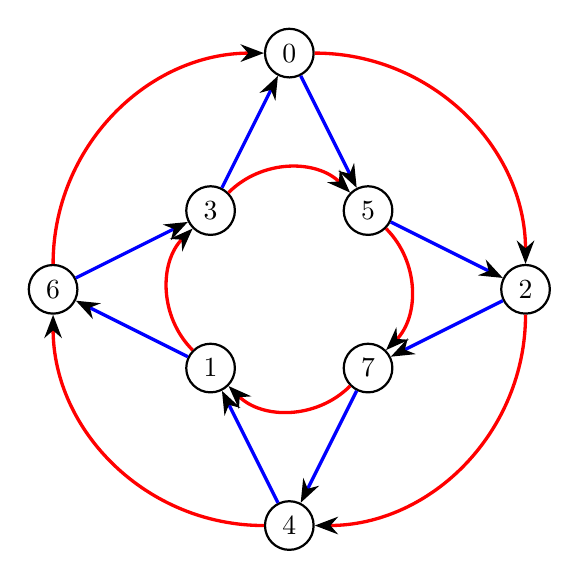
\begin{tikzpicture}
		\begin{scope}[every node/.style={circle,thick,draw}]
			\node(0) at (0,0)    {0};
			\node(1) at (-1,-4)  {1};
			\node(2) at (3,-3)   {2};
			\node(3) at (-1,-2)  {3};
			\node(4) at (0,-6)   {4};
			\node(5) at (1,-2)   {5};
			\node(6) at (-3,-3)  {6};
			\node(7) at (1,-4)   {7};
		\end{scope}
		\begin{scope}[>={Stealth[black]},
		every node/.style={fill=white,circle},
		every edge/.style={draw=red,very thick}]
			\path [->] (0) edge[bend left=45] (2);
			\path [->] (2) edge[bend left=45] (4);
			\path [->] (4) edge[bend left=45] (6);
			\path [->] (6) edge[bend left=45] (0);
			
			\path [->] (3) edge[bend left=45] (5);
			\path [->] (5) edge[bend left=45] (7);
			\path [->] (7) edge[bend left=45] (1);
			\path [->] (1) edge[bend left=45] (3);
			
		\end{scope}
		
		\begin{scope}[>={Stealth[black]},
		every node/.style={fill=white,circle},
		every edge/.style={draw=blue,very thick}]
			\path [->] (2) edge (7);
			\path [->] (5) edge (2);
			
			\path [->] (0) edge (5);
			\path [->] (3) edge (0);
			
			\path [->] (6) edge (3);
			\path [->] (1) edge (6);
			
			\path [->] (4) edge (1);
			\path [->] (7) edge (4);
			
		\end{scope}
		\end{tikzpicture}
	\item[7.18] Draw digraphs for the two possible structurally different groups of order 4.
	\item[]
	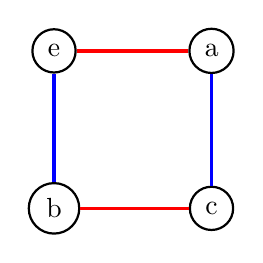
\begin{tikzpicture}
		\begin{scope}[every node/.style={circle,thick,draw}]
		\node(e) at (0,0)    {e};
		\node(b) at (0,-2)   {b};
		\node(a) at (2,0)   {a};
		\node(c) at (2,-2)  {c};
		\end{scope}
		\begin{scope}[>={Stealth[black]},
		every node/.style={fill=white,circle},
		every edge/.style={draw=red,very thick}]
		\path [-] (e) edge (a);
		\path [-] (b) edge (c);
		\end{scope}
		
		\begin{scope}[>={Stealth[black]},
		every node/.style={fill=white,circle},
		every edge/.style={draw=blue,very thick}]
		\path [-] (e) edge (b);
		\path [-] (c) edge (a);
		\end{scope}
	\end{tikzpicture}
	
	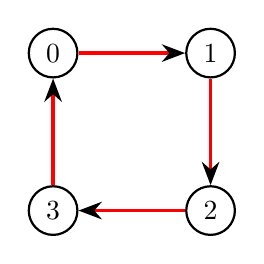
\begin{tikzpicture}
		\begin{scope}[every node/.style={circle,thick,draw}]
		\node(0) at (0,0)    {0};
		\node(1) at (2,0)    {1};
		\node(2) at (2,-2)   {2};
		\node(3) at (0,-2)   {3};
		\end{scope}
		\begin{scope}[>={Stealth[black]},
		every node/.style={fill=white,circle},
		every edge/.style={draw=red,very thick}]
		\path [->] (0) edge (1);
		\path [->] (1) edge (2);
		\path [->] (2) edge (3);
		\path [->] (3) edge (0);
		\end{scope}
	\end{tikzpicture}
	
	\item[8.02]
	
	\item[8.04]
	
	\item[8.08]
	
	\item[8.12]
	
	\item[8.18]
	
	\item[8.20]
	
	\item[8.28]

	\item[8.29]

	\item[8.36]

	\item[8.38]

	\item[8.46]

	\item[8.48]

	\item[8.50]
	
\end{enumerate}
\end{document}
